\documentclass[12pt]{article}

\setlength{\topmargin}{-.75in} \addtolength{\textheight}{2.00in}
\setlength{\oddsidemargin}{.00in} \addtolength{\textwidth}{.75in}

\usepackage{amsmath,color,graphicx,array,multirow,rotating, enumerate}
\usepackage{type1cm}
\usepackage{eso-pic}
\usepackage[hmargin=2cm,vmargin=1.3cm]{geometry}
\usepackage{mathabx}
\usepackage[rflt]{/Users/jgates/desktop/latex/floatflt}
\usepackage[table]{xcolor}
\nofiles

\def\Tab#1{\tabular[t]{>{\rule[-1ex]{0pt}{3ex}}c}#1\endtabular}
\newcolumntype{C}{@{}c@{}}

\pagestyle{empty}
\newcounter{ProbNum}
\setlength{\parindent}{0in}

% Watermark: graph paper
\newcommand\BackgroundPic{
\put(0,0){
\parbox[b][\paperheight]{\paperwidth}{%
\vfill
\centering
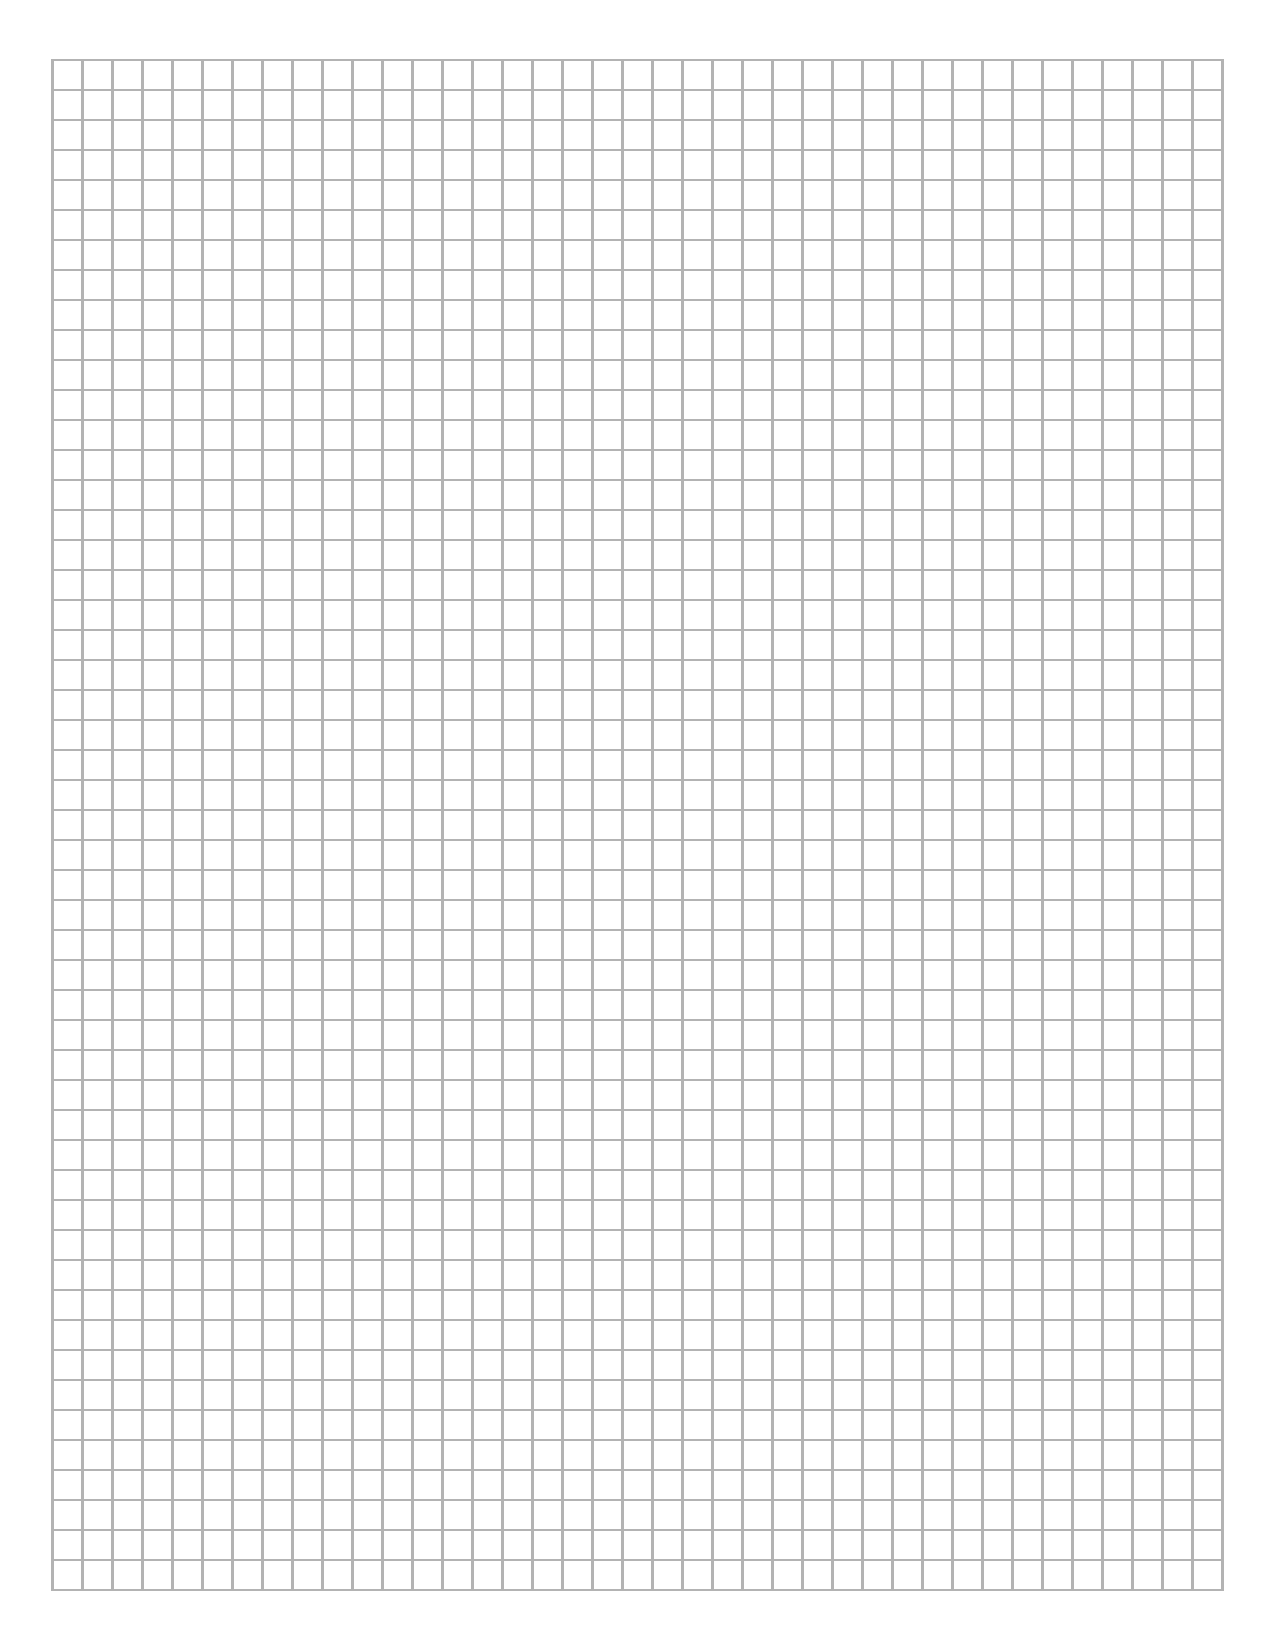
\includegraphics[width=\paperwidth,height=\paperheight,keepaspectratio]{/Users/jgates/desktop/latex/pics/plain.pdf}%
\vfill
}}}

%Diagram box command [v space][content]
\newcommand{\diagrambox}[2][40 mm]{
\framebox{\parbox{175 mm}{#2 \hfill \\ \vspace{#1}}}

\bigskip
}

% MakeList: [example number] [content]
\newcommand{\MakeList}[2]{
\begin{enumerate}[#1] \itemsep1pt \parskip0pt \parsep0pt  

#2
\end{enumerate}
}

\begin{document}



{\Large Problems tagged with standards:}BFPM
\bigskip 
% Number 1
% BFPM Tension FBD Vectors
% Hanging box, rope around 2 pulleys, theta = phi

\begin{floatingfigure}[r]{.2\textwidth}
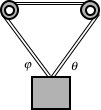
\includegraphics[scale=1]{/Users/jgates/desktop/latex/pics/hangingbox1.png}
\end{floatingfigure}
 
{\bf \Large{1.}} The box of mass ${6~kg}$ hangs at rest. 

\bigskip

\indent  a. Prove that ${\theta = \varphi}$.

\vfill

b. Determine the tension in the rope, if ${\theta = 50^\circ}$.

\vfill

\newpage
% Number 50
% UFPM GM UCM
% Simple circular orbit - geosynch

{\bf \Large{5.}} ${\left ( G = 6.67 \times 10^{-11}~\tfrac{Nm^2}{kg^2} \right )}$ A satellite is said to be in \emph{geosynchronous orbit} if it always stays above the same spot on the body that it is orbiting.  It accomplishes this by having the same orbital period as the rotational period of the body that is it orbiting. (How long is that for the Earth?)

\bigskip

a. Determine how far from the surface of the Earth a satellite must be placed in order to be in a geosynchronous orbit. ${\left ( R_{\Earth} = 6,370~km; M_{\Earth}=5.97 \times 10^{24}~kg \right )}$

\vfill

b. The space shuttle orbits the Earth with a period of around 90 minutes.  Is it closer to the Earth or further from the Earth than geosynchronous satellites?  Be convincing!

\vspace{25mm}
 
\newpage
\end{document}